\chapter{Proposed conditioned object detector}
\label{ch:cod}
As discussed in Section \ref{sec:motivation}, this thesis proposes a modular approach to solve the Visual-Conditioned Multi-Task Imitation Learning Problem. This chapter focuses on the module responsible for addressing an instance of the ``Cognitive Task" relevant to the context under consideration. Specifically, the approach aims to leverage an \textbf{object-prior} to enable the system to ignore distractor objects in the scene and focus on the target region of interest. To achieve this goal, a preliminary step is to develop a system capable of computing this object-prior. Therefore, this chapter will present and discuss the design of the Conditioned Object Detector (COD), which is specifically designed to solve a \textbf{novel variation} of the well-known Object Detection problem. Unlike traditional object detection tasks, where a deep architecture produces bounding boxes for all objects in the scene, this variation requires generating bounding boxes only for the regions of interest based on the demonstrated task.

Section \ref{sec:cod_related_works} will review relevant methods related to this task. 
Section~\ref{sec:cod_problem} outlines the detection problem being addressed. Section~\ref{sec:cod_architecture} describes the proposed architecture for solving this problem. Finally, Section~\ref{sec:cod_experimental} discusses the experimental setup and presents the results obtained from testing the proposed architecture.

\section{Related Works}
\label{sec:cod_related_works}
This section will review the preliminary research conducted in the context of Object-Oriented Imitation Learning (Section \ref{sec:ooil}) to understand how previous studies have leveraged object priors to solve the Learning from Demonstration (LfD) problem. Additionally, it will examine research in the context of Visual-Question Answering (Section \ref{sec:vqa}) to highlight the specific challenges addressed by the COD module, while also presenting the methods that have primarily inspired the proposed solution.

\subsection{Object-Oriented Imitation Learning}
\label{sec:ooil}
All the methods discussed in Section \ref{sec:lfd} share a common characteristic: they are end-to-end systems that take high-level inputs, such as images, and directly generate the corresponding actions as output. While this approach can be sufficient in scenarios where the scene is simple, meaning there are no distracting objects, or if there are distracting objects, they can be easily identified by the system because they are consistently not involved in the manipulation, this end-to-end approach may struggle in more complex environments. Specifically, it can encounter difficulties when the robot workspace contains objects that are similar to each other, especially if these objects are involved in manipulation for some task variations.

Based on this consideration, this paragraph will describe methods that leverage object priors. This means that the control policy is informed not only by the embedding of the agent scene, which is obtained from a deep architecture, but also by object-level information, such as the bounding boxes of objects in the scene, obtained from an object detector.

The concept of leveraging object priors has been explored in both earlier works \cite{devin2018deep,park2021object} and more recent approaches \cite{belkhale2023plato,zhu2023viola,zhu2023learning,jiang2023vima}.

One of the preliminary works on leveraging object priors was presented by the authors of \cite{devin2018deep}. This work primarily focuses on the challenge of generalization in Learning from Demonstration (LfD) systems that use an end-to-end approach. In such systems, a task-specific model is trained to predict actions based on raw visual observations. The authors found that while it is possible to achieve good \textit{instance-level generalization}, meaning the model can solve tasks with varying initial configurations using a limited number of samples, achieving \textit{category-level generalization} is more challenging. Category-level generalization refers to the model ability to solve tasks involving different objects. To achieve this, the dataset must include a large number of trajectories involving a wide variety of objects. For instance, if the task is to pour the contents of a bottle into a cup, the dataset should contain trajectories with different types of cups and bottles. However, constructing such a dataset is time-consuming and costly. Moreover, the potential of well-known large datasets in classical computer vision tasks, such as object detection, is not fully utilized.

To address this issue, the authors proposed a paradigm shift by introducing a robotic vision framework that operates on sets of objects rather than raw pixel data. This framework leverages prior datasets to learn a generic object concept model, thereby enhancing category-level generalization without requiring an extensive and diverse dataset. The framework is illustrated in Figure \ref{fig:object_prior_framework} and is composed of several stages:
\begin{itemize}
    \item \textbf{Meta-Attention}, which is basically a Region Proposal Network (RPN) \cite{fastrcnn}, trained on the well known MSCOCO \cite{lin2014microsoft} dataset. The RPN generates objects proposals, i.e., region of the image that possibly contain an object.
    \item \textbf{Task-Specific Attention}, which aims to learn what are the object of interest with respect to the task in hand. This module is parameterized as a vector $w$ such that the attention paid to $o^i$ is proportional to $e^{w^Tf(o^i)}$.
    \item \textbf{Soft Attention}, this module gives a probabilistic meaning to the attention map obtained from the Task-Specific Attention. Specifically, a Boltzmann distribution is used to map the attention weights to a probability for each object proposal, i.e., $p\left(o^i \mid w_j\right)=\frac{e^{w_j^{\top} \frac{f\left(o^i\right)}{\left\|f\left(o^i\right)\right\|_2}}}{\sum_{i=0}^N e^{w_j^{\top} \frac{f\left(o^i\right)}{\left\|f\left(o^i\right)\right\|_2}}}$.
    \item \textbf{Movement Prediction Network}, this module predicts the next robot action, given the attended object information from the soft attention, and the robot state represented by the joint and end-effector state.
\end{itemize}
\begin{figure}[t]
    \centering
    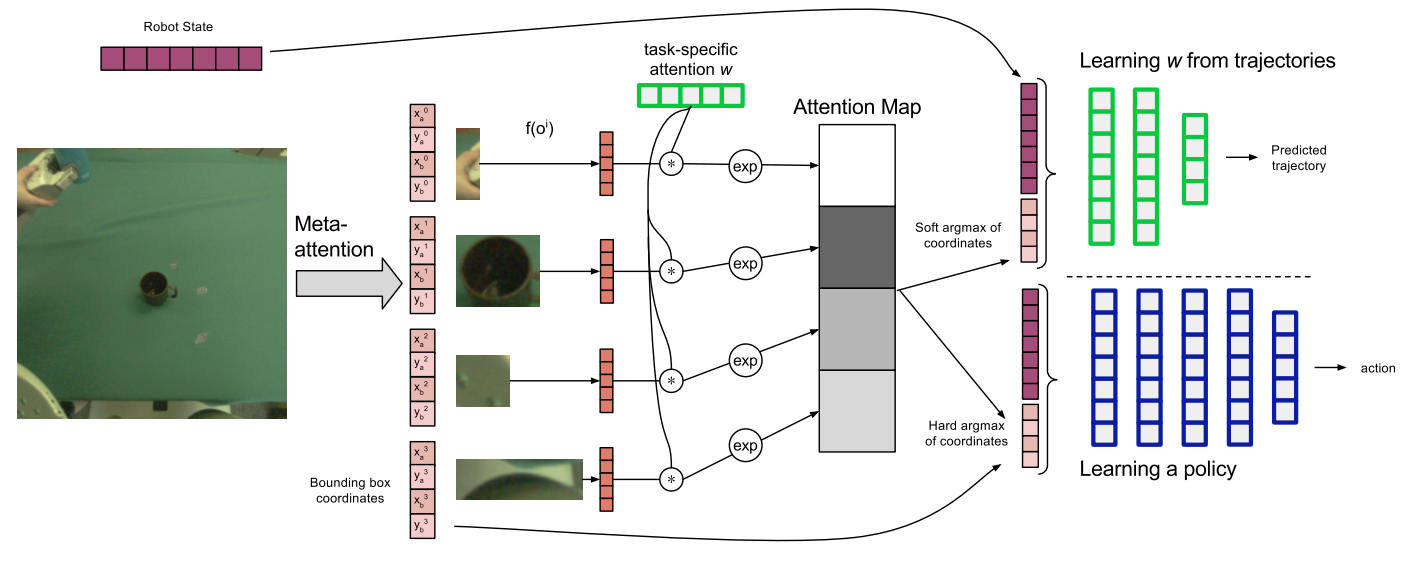
\includegraphics[width=0.8\textwidth]{figures/images/object_prior_framework.png}
    \caption{
            Robotic vision framework proposed in \cite{devin2018deep}. The framework is divided into different stages: \textbf{Meta-Attention}: Generates object proposals from an input image, trained on an object detection dataset, and shared across tasks; \textbf{Task-Specific Attention}: Focuses on relevant objects for a task using the meta-attention's semantic features; \textbf{Soft Attention}: Distributes attention as probabilities over object proposals using a Boltzmann distribution; \textbf{Movement Prediction Network}: Combines attended object information with the robot's state to predict the next action.
        }
    \label{fig:object_prior_framework}
\end{figure}
This preliminary work focused mainly on two tasks:
\begin{itemize}
    \item  \textit{Pouring Task}: The robot is required to pour contents from a bottle into a mug. The challenge is to locate the mug from an image without being explicitly provided its location, especially when different mugs are used during training and testing.
    \item \textit{Sweeping Task}: The robot must sweep an object (e.g., a plastic orange) into a dustpan, with both objects starting in different positions. This task requires the robot to adapt its approach based on the relative positions of the objects.
\end{itemize}
During testing, the authors focused on \textit{Category Generalization} and the ability to \textit{Ignore Distractor Objects}. For the former, the system was trained with only one type of mug and evaluated with other mugs (Figure \ref{fig:pouring_task_setting}). The results showed that the system successfully poured the contents into the correct mug, thanks to the learned task-specific attention weight that highlighted the mug features. For the latter, the authors designed a test where two mugs were present in the scene (Figure \ref{fig:task_specific_attention}). Since the model did not receive any conditioning signal indicating which mug to use, the authors fine-tuned the attention weight on trajectories where only the brown mug was used, demonstrating that this mechanism could focus on more specific features, such as the mug color.
\begin{figure}[t]
    \centering
    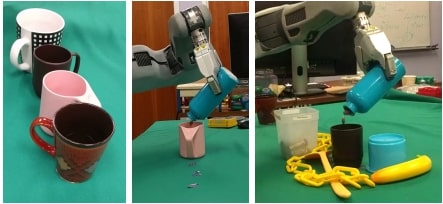
\includegraphics[width=0.6\textwidth]{figures/images/deep_object_centric_representation/pouring_task.jpg}
    \caption{Pouring task setting proposed in \cite{devin2018deep}. (Left) Mugs used for evaluation. Note that only the brown mug was seen during training. Center: Successful pouring into the pink mug. (Right) Pouring into the brown mug in a cluttered environment that was not seen during training.}
    \label{fig:pouring_task_setting}
\end{figure}

\begin{figure}[t]
    \centering
    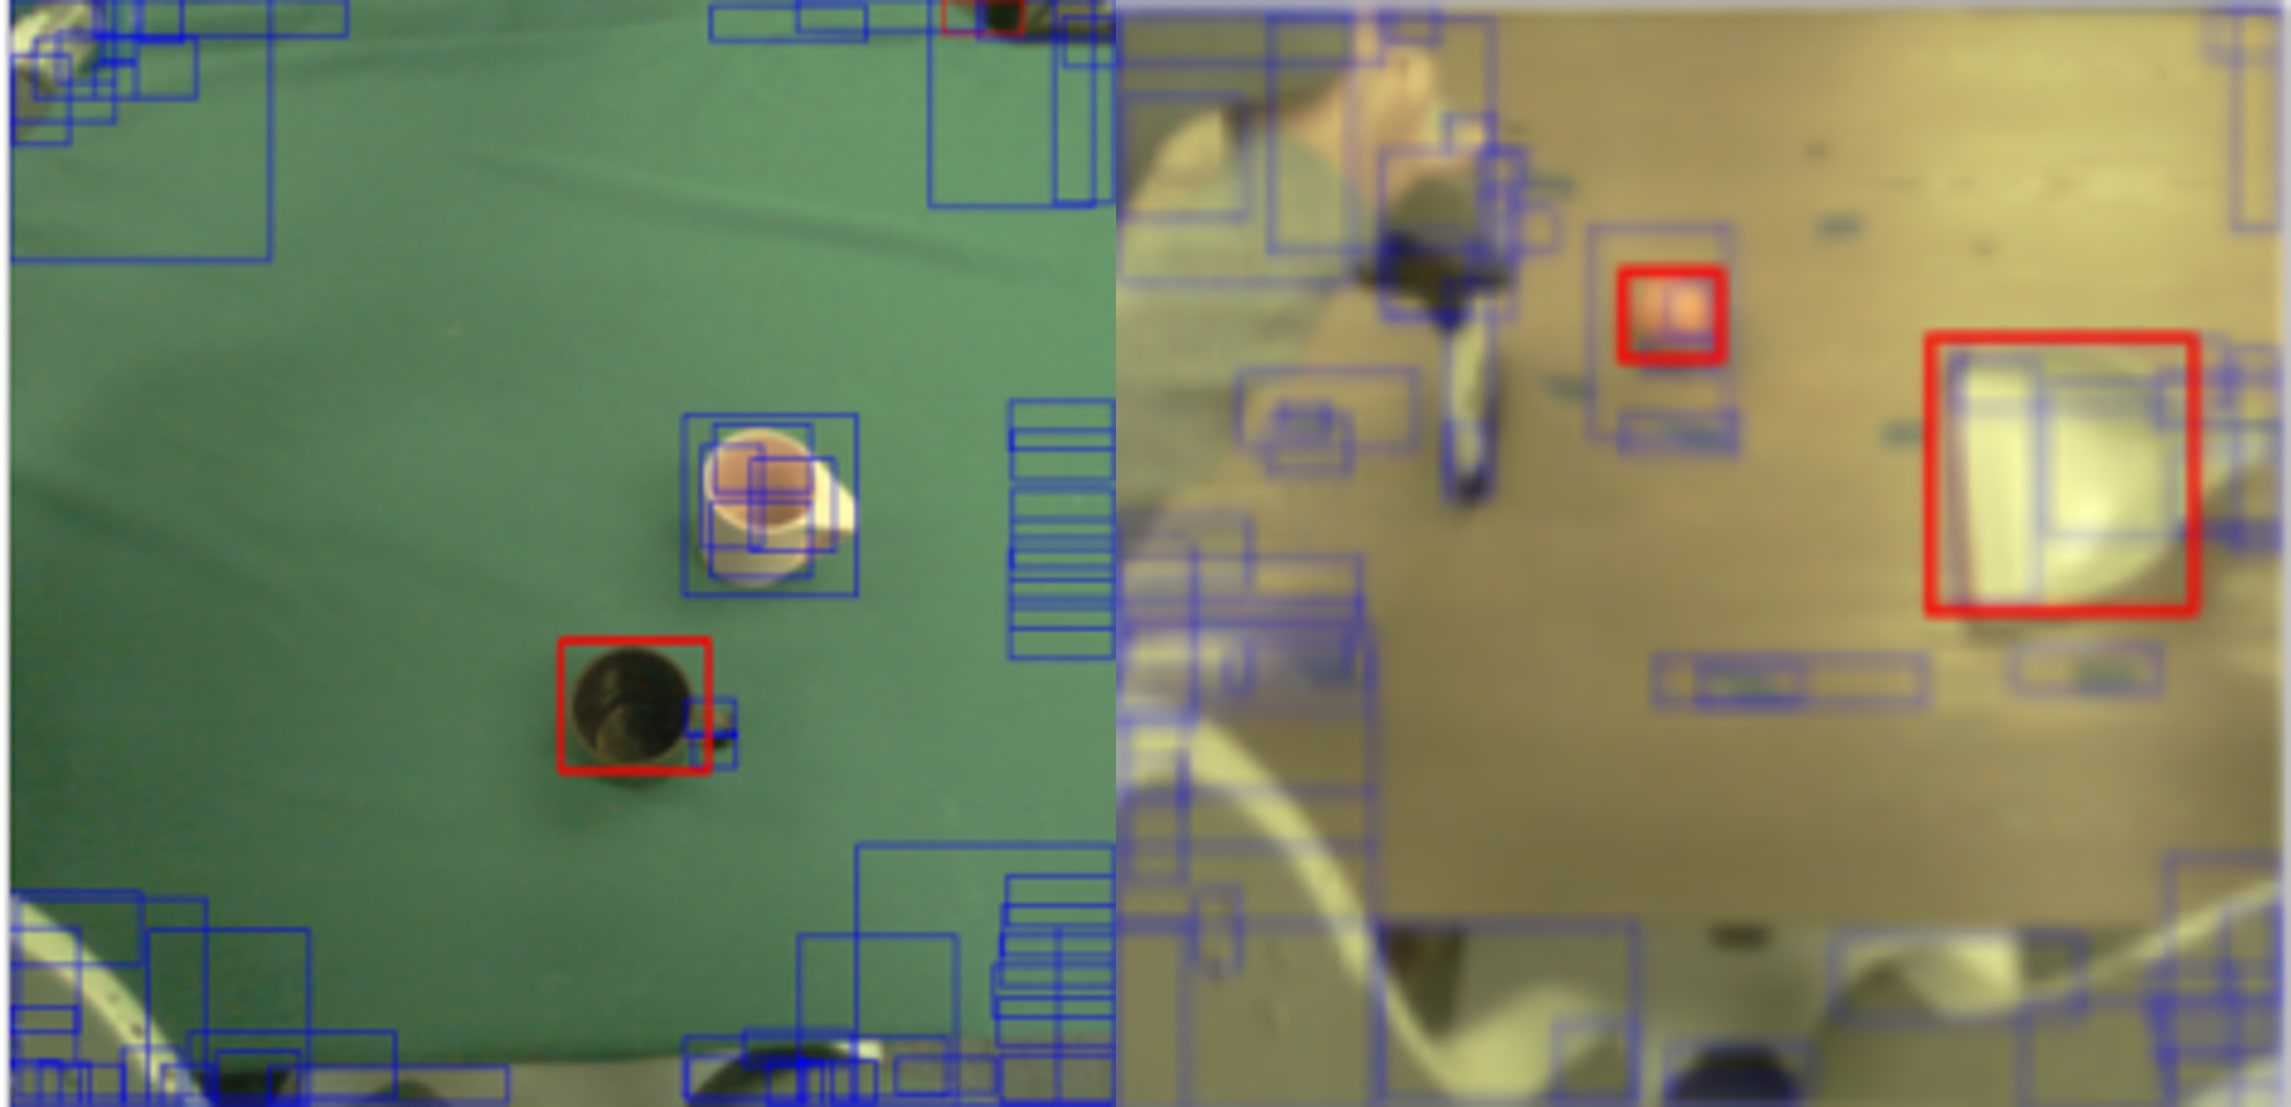
\includegraphics[width=0.6\textwidth]{figures/images/deep_object_centric_representation/mugs_distractors.jpg}
        \caption{The region proposals (meta-attention) are drawn in blue and the task-specific attended regions are drawn in red. For the Pouring task with distractor mug (pink) and target mug (brown), the attention locks on to the brown mug as its position defines the trajectory. For the sweeping task, two attention vectors are used, one attends to the orange and one attends to the dustpan.}
    \label{fig:task_specific_attention}
\end{figure}

In summary, this preliminary work demonstrated that leveraging object priors can facilitate category-level generalization by utilizing large, well-known datasets for the object-detection problem. However, the experimental setup was relatively simple, even in scenarios with distractor objects. The proposed system could handle distractor objects only after specific fine-tuning and was not able to dynamically discriminate between objects of interest and distractors based on task variations.

A recent work that follows a similar approach is proposed in \cite{zhu2023viola}. In this work, the authors introduced VIOLA (Visuomotor Imitation via Object-centric Learning) (Figure \ref{fig:viola_architecture}), an architecture inspired by the ideas presented in \cite{devin2018deep}. VIOLA uses an RPN and a ResNet18 \cite{resnet} to generate object proposals and produce a spatial feature map, respectively. It then constructs a \textit{per-step feature} vector, composed of three key elements: a \textbf{global context feature} that encodes the current task stage, an \textbf{eye-in-hand visual feature} to mitigate occlusion, and a \textbf{proprioceptive feature} that captures the robot state. These per-step features are concatenated to form a \textbf{history of observations}, which is designed to capture temporal dependencies and dynamic changes in object states. This tensor is then fed into a Transformer \cite{vaswani2017attention}, which leverages its intrinsic attention mechanism to automatically focus on the object of interest.
\begin{figure}[t]
    \centering
    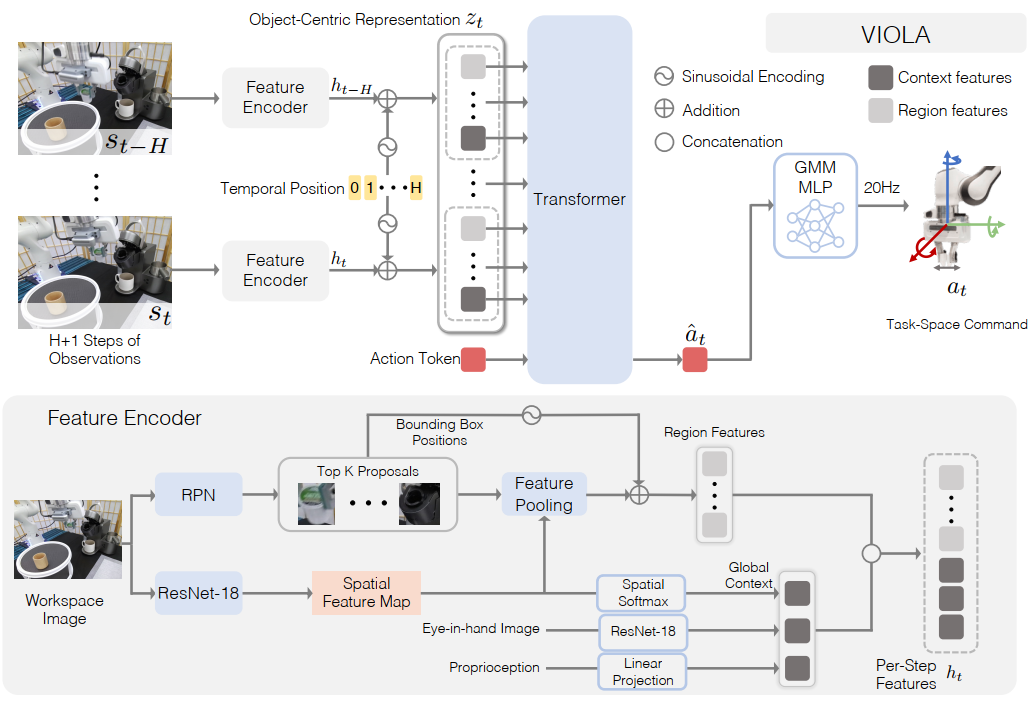
\includegraphics[width=0.7\textwidth]{figures/images/viola/viola_architecture.png}
        \caption{The VIOLA architecture proposed in \cite{zhu2023viola}. (Top) The overall control architecture is based on a Transformer module that processes a stack of \textit{per-step features} $h_{t}$, obtained from the Feature Encoder, to generate a final action embedding, which is then input into a GMM policy. (Bottom) The Feature Encoder builds both local and global features. Local features correspond to regions of interest extracted by the RPN. Global features are obtained by processing the workspace image, the image from the camera on the gripper, and proprioceptive information.
        }
    \label{fig:viola_architecture}
    
\end{figure}

\begin{figure}[t]
    \centering
    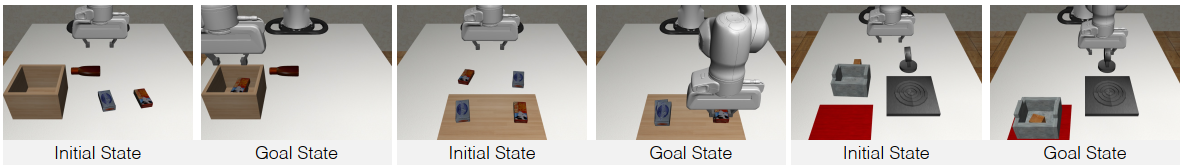
\includegraphics[width=0.9\textwidth]{figures/images/viola/viola_task.png}
    \caption{Simulation tasks on which the VIOLA \cite{zhu2023viola} method was tested. (Left) Sorting task. (Center) Stacking task. (Right) BUDS-Kitchen task}
    \label{fig:viola_task}
    
\end{figure}

This method was first evaluated in a simulation environment across three tasks, as depicted in Figure \ref{fig:viola_task}. Various testing scenarios were considered, including different object placements, the introduction of distractor objects, and changes in camera position. Generally speaking, VIOLA outperformed all baselines across these testing conditions, further demonstrating the utility of object priors in enhancing the robustness of such methods. However, similar to \cite{devin2018deep}, the testing scenarios were relatively simple, with clear distinctions between distractors and objects of interest. The distractors were objects never seen during the demonstration and were not involved in manipulation, making them relatively easy for the model to discriminate.

In the works discussed so far, the approach has primarily focused on leveraging object priors to directly predict the actions that the robot must perform. However, a different approach was proposed in \cite{belkhale2023plato}, where the authors introduced an alternative interpretation of object-centric concept. Instead of focusing on the robot perspective, they shifted the emphasis to the object perspective, proposing PLATO (Predicting Latent Affordances Through Object-Centric Play). PLATO is a learning framework that learns a \textbf{latent affordance space}, which describes how an object can be used (e.g., a block being grasped, a door knob being turned, or a drawer being opened).

The authors argue that learning these affordances (i.e., what happens to the object) rather than plans (i.e., what happens to the robot) from play leads to a simpler and more robust task representation that can operate over varying time horizons. This, in turn, results in more effective policies at test time. This paradigm shift allows the policy to reason about the environment more effectively: given access to an affordance (e.g., the door knob being turned) and a goal (e.g., an opened door), the policy can work backwards to infer the behavior needed to exploit that affordance (e.g., reaching the knob and rotating the gripper to turn it).

To reach this objective authors started from the observation that a single-object manipulation is composed of the following three phases:
\begin{enumerate}
    \item \textbf{Pre-interaction}, when the robot prepares to interact with an object (e.g., reaching for a block).
    \item \textbf{Interaction}, when the robot and the object engage in joint actions (e.g., pushing or pulling the block).
    \item \textbf{Post-interaction}, when the robot separates from the object, and the object may come to rest (e.g., the block stops moving).
\end{enumerate}
Given these three phases, the algorithm learns a \textbf{latent affordance distribution}. Specifically, the architecture comprises three learnable modules:  $E$,  $E'$, and  $\pi$.  $E$ models the posterior distribution, mapping the full interaction trajectory  $\tau^{i}$ to the corresponding latent affordance distribution, from which the affordance embedding  $z$ is sampled.  $E'$ is the prior module used during rollout. It takes the current state and the goal state as input and generates the affordance embedding  $z'$. This module is trained to match the posterior distribution modeled by  $E$.  $\pi$ represents the current policy, which generates the action  $a^{i}$ given the current state  $s^{i}$, the desired goal  $o_g$, and the latent embedding  $z$.

These three modules are trained end-to-end by minimizing the loss function in Formula \ref{eq:plato_equation}, which includes three terms. The first two terms correspond to the policy  $\pi$, ensuring it matches the ground-truth trajectories in the interaction and pre-interaction phases. The last term is the KL-divergence, used to train the posterior and prior modules  $E$ and  $E'$.

\begin{equation}
    \label{eq:plato_equation}
    \begin{aligned}
        \mathcal{L}_{PLATO} = -\log \left(\pi\left(a_{1: H}^{(i)} \mid s_{1: H}^{(i)}, o_g, z\right)\right)- \\ 
        \alpha \log \left(\pi\left(a_{1: H}^{(-)} \mid s_{1: H}^{(-)}, o_g, z\right)\right)+ \\ 
        \beta \operatorname{KL}\left(p(z) \| p\left(z^{\prime}\right)\right)
    \end{aligned}
\end{equation}
\begin{figure}[t]
    \centering
    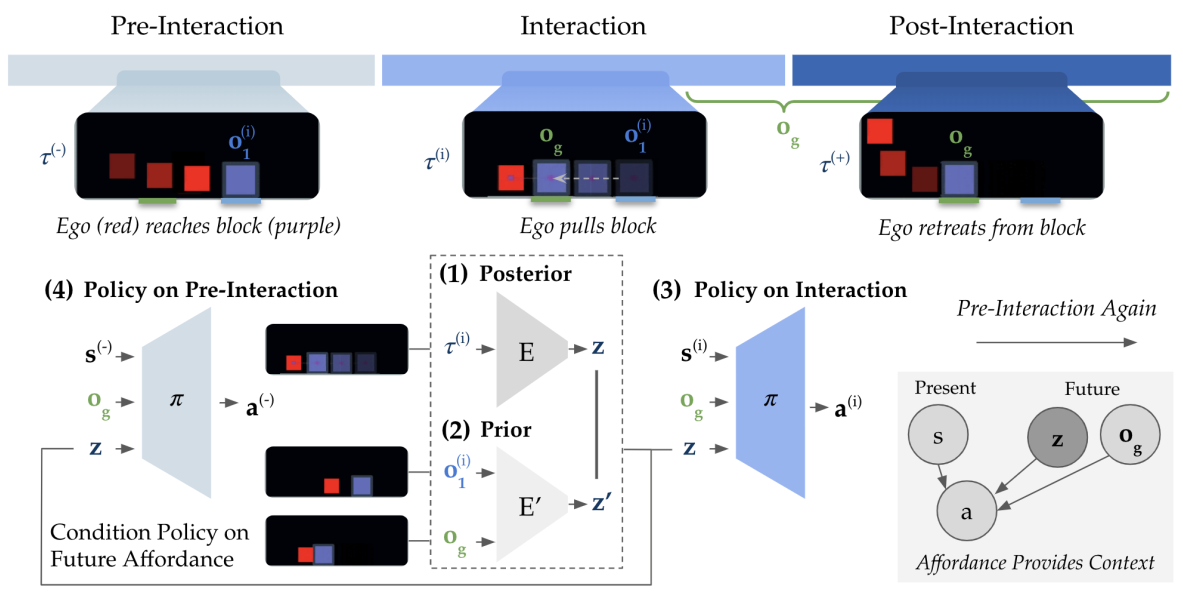
\includegraphics[width=0.7\textwidth]{figures/images/plato/plato.png}
    \caption{PLATO architecture proposed in \cite{belkhale2023plato}. The architecture is composed of different stages. (1) The posterior encoder \( E \) encodes the interaction sequence \( \tau^{(i)} \) into the affordance \( z \). (2) The prior encoder \( E' \) encodes the object initial state \( o^{(i)}_1 \) and goal state \( o_g \) to predict \( z \), with \( o_g \) sampled after the interaction. (3) The policy is trained to output actions during the interaction period conditioned on the affordance. Simultaneously, (4) it is trained to output actions during the pre-interaction period conditioned on the ``future" affordance.
    }
    \label{fig:plato}
    
\end{figure}

\begin{figure}[t]
    \centering
    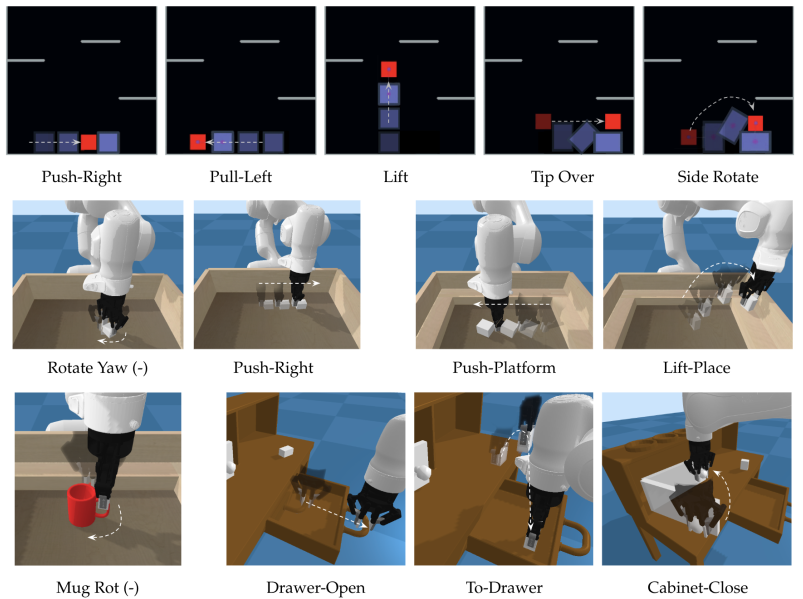
\includegraphics[width=0.7\textwidth]{figures/images/plato/tasks.png}
    \caption{ Testing scenarios and primitives proposed in \cite{belkhale2023plato}. (Top) \textbf{Block2D} Environment primitive examples. (Center) \textbf{Block3D} and \textbf{Block3DPlatform} primitive examples. (Bottom) The left image shows an example primitive in \textbf{Mug3D-Platforms}. The right three images show sample tasks from \textbf{Playroom3D}.}
    \label{fig:plato_task}
    
\end{figure}

Finally, this method was tested in a variety of scenarios, including both single-object and multiple-object manipulation with different manipulation primitives (Figure \ref{fig:plato_task}). However, in the multi-object scenarios, the system was only tested on single-object manipulation primitives.

This work is particularly noteworthy as it demonstrates that a policy can be learned by solving an inverse problem, starting from object affordances and deriving the corresponding robot trajectories. It also shows that the policy can be conditioned based on the desired goal state. However, certain aspects were not addressed in this work, such as the potential presence of distractor objects and tasks requiring the manipulation of multiple objects. Additionally, the affordances were learned in the object space (i.e., with known object poses) rather than in the high-level image space.

The works discussed in this paragraph highlight the significant research efforts aimed at modeling the manipulation problem from an object-centric perspective. These efforts either focus on the affordances of the object (i.e., the possible movements the object allows) or introduce object priors defined by regions of interest that may contain the object to be manipulated, with results demonstrated in both simulated and real-world environments. However, the methods presented so far primarily address single-task scenarios, where distractor objects can be easily identified as they remain constant across demonstrations. In contrast, this thesis proposes a solution for a more challenging scenario in which the robot operates in a multi-variation environment. This environment includes multiple similar objects, which may serve as either targets or distractors depending on the specific task variation.

\subsection{Visual-Question Answering}
\label{sec:vqa}
The \textit{Visual-Question Answering} (VQA) problem refers to the ability of a system of ``reasoning'' over an image, based on a given query expressed in terms of text. This means that, given in input an arbitrary image and an arbitrary textual prompt the system must be able to generate an answer to the given prompt (Figure \ref{fig:vqa_example}).
\begin{figure}[t]
    \centering
    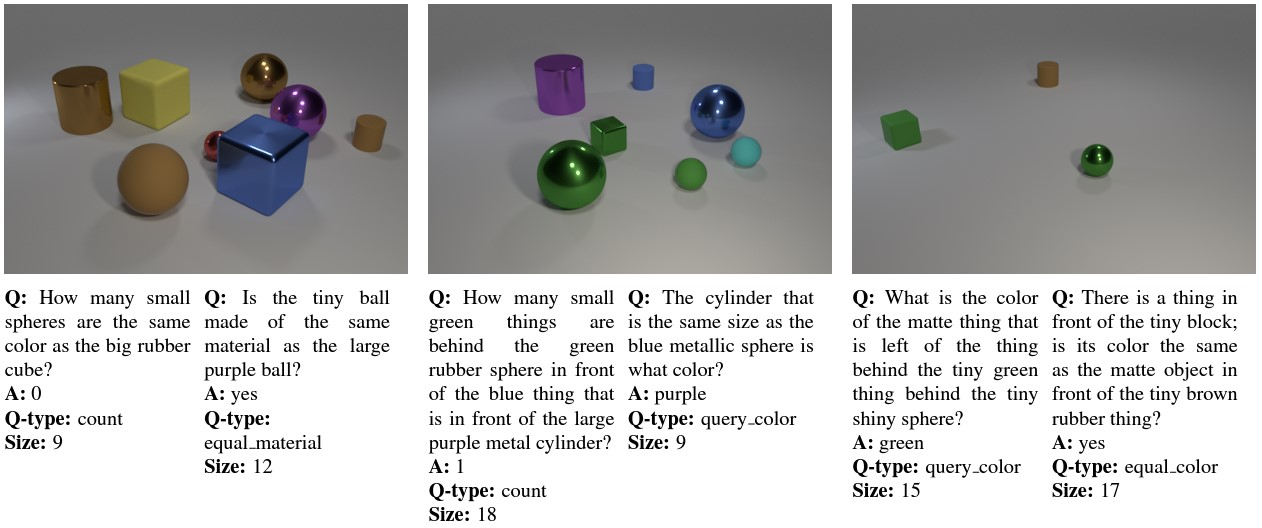
\includegraphics[width=1.0\textwidth]{figures/images/ch2/vqa_problem.jpg}
    \caption{Example of Vision-Question Answering problem get from the CLEVR \cite{johnson2017clevr} dataset. It is possible to observe how for a given image multiple different questions can be done. As well as, questions covers different reasoning skills such as attribute identification, counting, comparison, multiple attention, and logical operations.}
    \label{fig:vqa_example}
\end{figure}


The key aspect related to this problem is related to the fact that for a given image different questions can be made. There is no predefined mapping between an input image and its corresponding answer. Instead, the system must dynamically adjust its \textbf{attention} to specific regions of the image based on the given query. This requires effectively \textbf{correlating} the image encoding with the prompt encoding to generate a conditioned embedding that can reliably produce a valid answer.

Based on these preliminary considerations, various solutions have been proposed using both Convolutional Neural Network architectures \cite{perez2018film} and novel Transformer architectures \cite{chen2022caan,chen2024mpcct,liu2024visual}.

A significant breakthrough in this field was introduced in \cite{perez2018film}, where the FiLM (Feature-wise Linear Modulation) conditioning layer was proposed. The core idea behind FiLM is to dynamically modify the output of a neural network by applying an affine transformation to its intermediate features based on some input. Specifically, the FiLM layer learns two functions, $f$ and $h$, which produce the coefficients $\gamma_{i,c}$ and $\beta_{i,c}$, respectively, based on an input $x_{i}$, as defined in Equation \ref{eq:film}.
\begin{equation}
    \label{eq:film}
    \begin{matrix}
        \gamma_{i,c} = f_{c}(x_{i}) & 
        \beta_{i,c} = h_{c}(x_{i})
    \end{matrix}
\end{equation}
These coefficients are then used to modulate the $c^{th}$ activation map $\textbf{F}_{i,c}$ through a \textit{feature-wise affine transformation}, as described in Equation \ref{eq:film_eq}.
\begin{equation}
    \label{eq:film_eq}
    FiLM(\textbf{F}_{c}|\gamma_{c}, \beta_{c}) = \gamma_{c} \textbf{F}_{c} + \beta_{c}
\end{equation}

An example of integrating the FiLM layer into a deep architecture is shown in Figure \ref{fig:film_architecture}, illustrating the implementation proposed in \cite{perez2018film}. In this configuration, the prompt is encoded using a Gated Recurrent Unit (GRU), and the resulting embedding is fed into a Multi-Layer Perceptron (MLP), which outputs the coefficients $\gamma_{i,c}$ and $\beta_{i,c}$. These coefficients are subsequently used to modulate the activations of $N$ Residual Blocks (ResBlocks).
\begin{figure}[t]
    \centering
    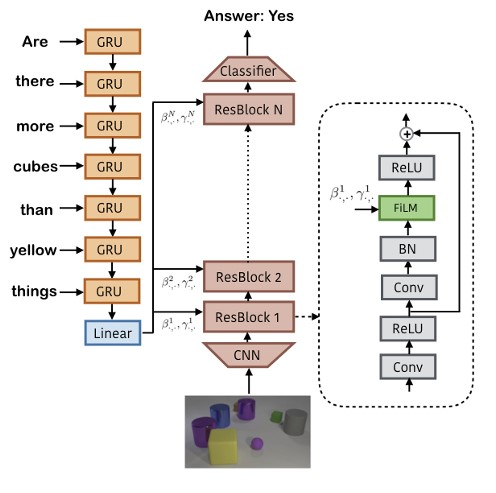
\includegraphics[width=0.6\textwidth]{figures/images/ch2/film_architecture.jpg}
    \caption{Proposed integration of the FiLM conditioning layer. Here, the Linear Modulation is applied to modify the activation maps of the ResNet blocks, while a linear layer generates the modulation coefficients $\beta$ and $\gamma$ based on the embedding derived from the textual prompt. This enables the model to conditionally adjust the activation maps according to the context provided by the input query}
    \label{fig:film_architecture}
\end{figure}


The FiLM layer has also been effectively applied in the context of Language-Conditioned Policy Learning (Section \ref{sec:occp_mtil}) \cite{jang2022bc_z,brohan2022rt}. Starting from a textual prompt describing a desired task, the FiLM layer modulates the activation maps of the convolutional blocks in the network that encodes the robot's observations. This allows the network to focus on specific parts of the image relevant to the task (Figure \ref{fig:film_attention}).
\begin{figure}[t]
    \centering
    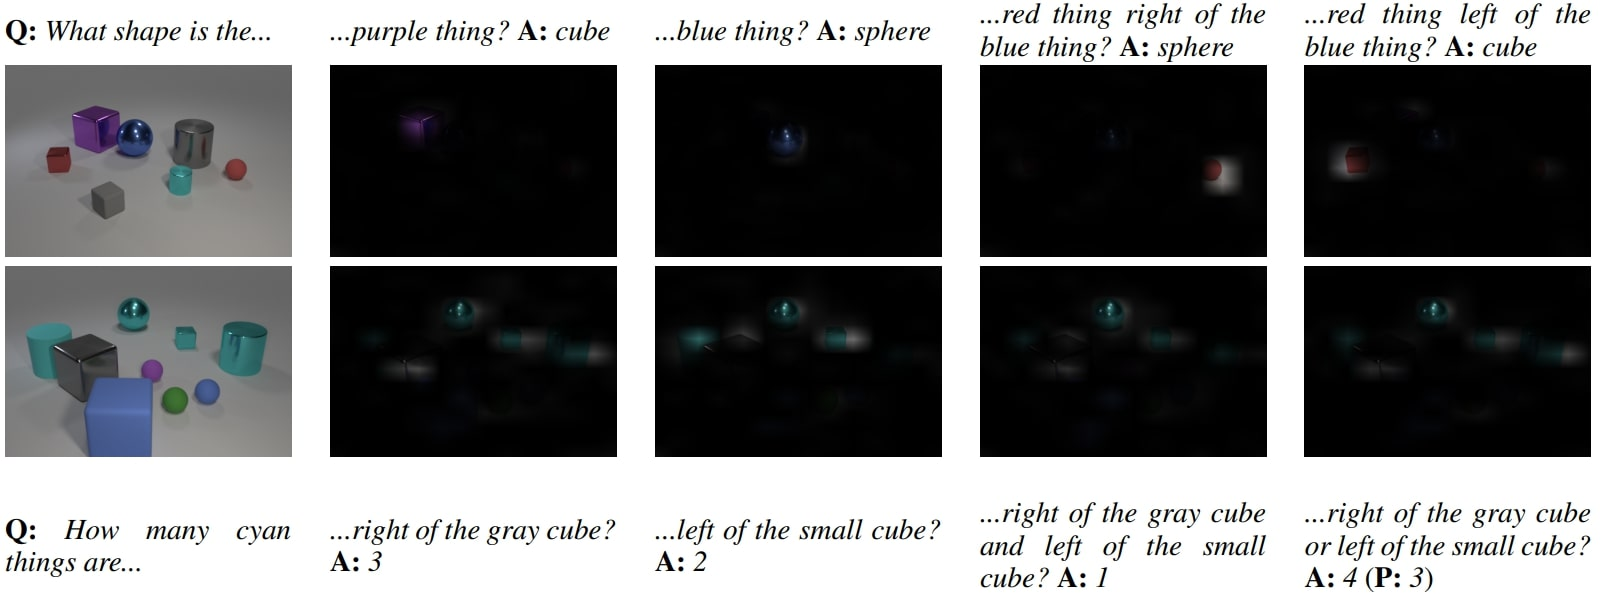
\includegraphics[width=0.9\textwidth]{figures/images/film/film_attention.jpg}
    \caption{Visualizations of the distribution of locations used by the model for its globally max-pooled features, from which its final MLP makes predictions. FiLM correctly localizes the object referenced by the answer (top) or all objects referenced by the question (bottom). However, the localization is less accurate when the model provides an incorrect answer (rightmost bottom).}
    \label{fig:film_attention}
\end{figure}


Since the introduction and expansion of Transformer models \cite{vaswani2017attention}, there has been a major shift towards solving the Visual Question Answering (VQA) problem by utilizing these architectures. Transformers excel at capturing intra-modal relationships through dependency modeling and promoting alignment and interaction between multiple modalities. This has led to the development of Vision-Language Transformers capable of directly processing multi-modal inputs, such as images and text. An example is the LLaVA model proposed in \cite{liu2024visual}, which represents the current state-of-the-art in VQA. However, despite its capability to handle complex queries, LLaVA relies on a Large Language Model (LLM) with a minimum size of 7 billion parameters, requiring a high-performance server. This makes real-time deployment in real-world systems, such as robotic control, challenging or even impractical.


\section{Problem formulation}
\label{sec:cod_problem}
\section{Architecture}
\label{sec:cod_architecture}
\section{Experiments}
\label{sec:cod_experimental}
In this section, the performed experiments are going to be described. Specifically, in  
Section~\ref{sec:cod_dataset} the dataset used for training procedure will be described. Section~\ref{sec:cod_results} will report the obtained results.
\subsection{Dataset}
\label{sec:cod_dataset}
To validate the proposed architecture, a simulated dataset was generated, focusing on four primary tasks: \textit{Pick-Place}, \textit{Nut-Assembly}, \textit{Stack-Block}, and \textit{Press-Button}. Each task consists of multiple variations. Specifically, the Pick-Place task has 16 variations, Nut-Assembly has 9 variations, Stack-Block has 6 variations, and Press-Button has 6 variations. Each task and its variations are graphically described in Figure~\ref{fig:dataset_cod}.
\begin{figure}[t]
    \centering
    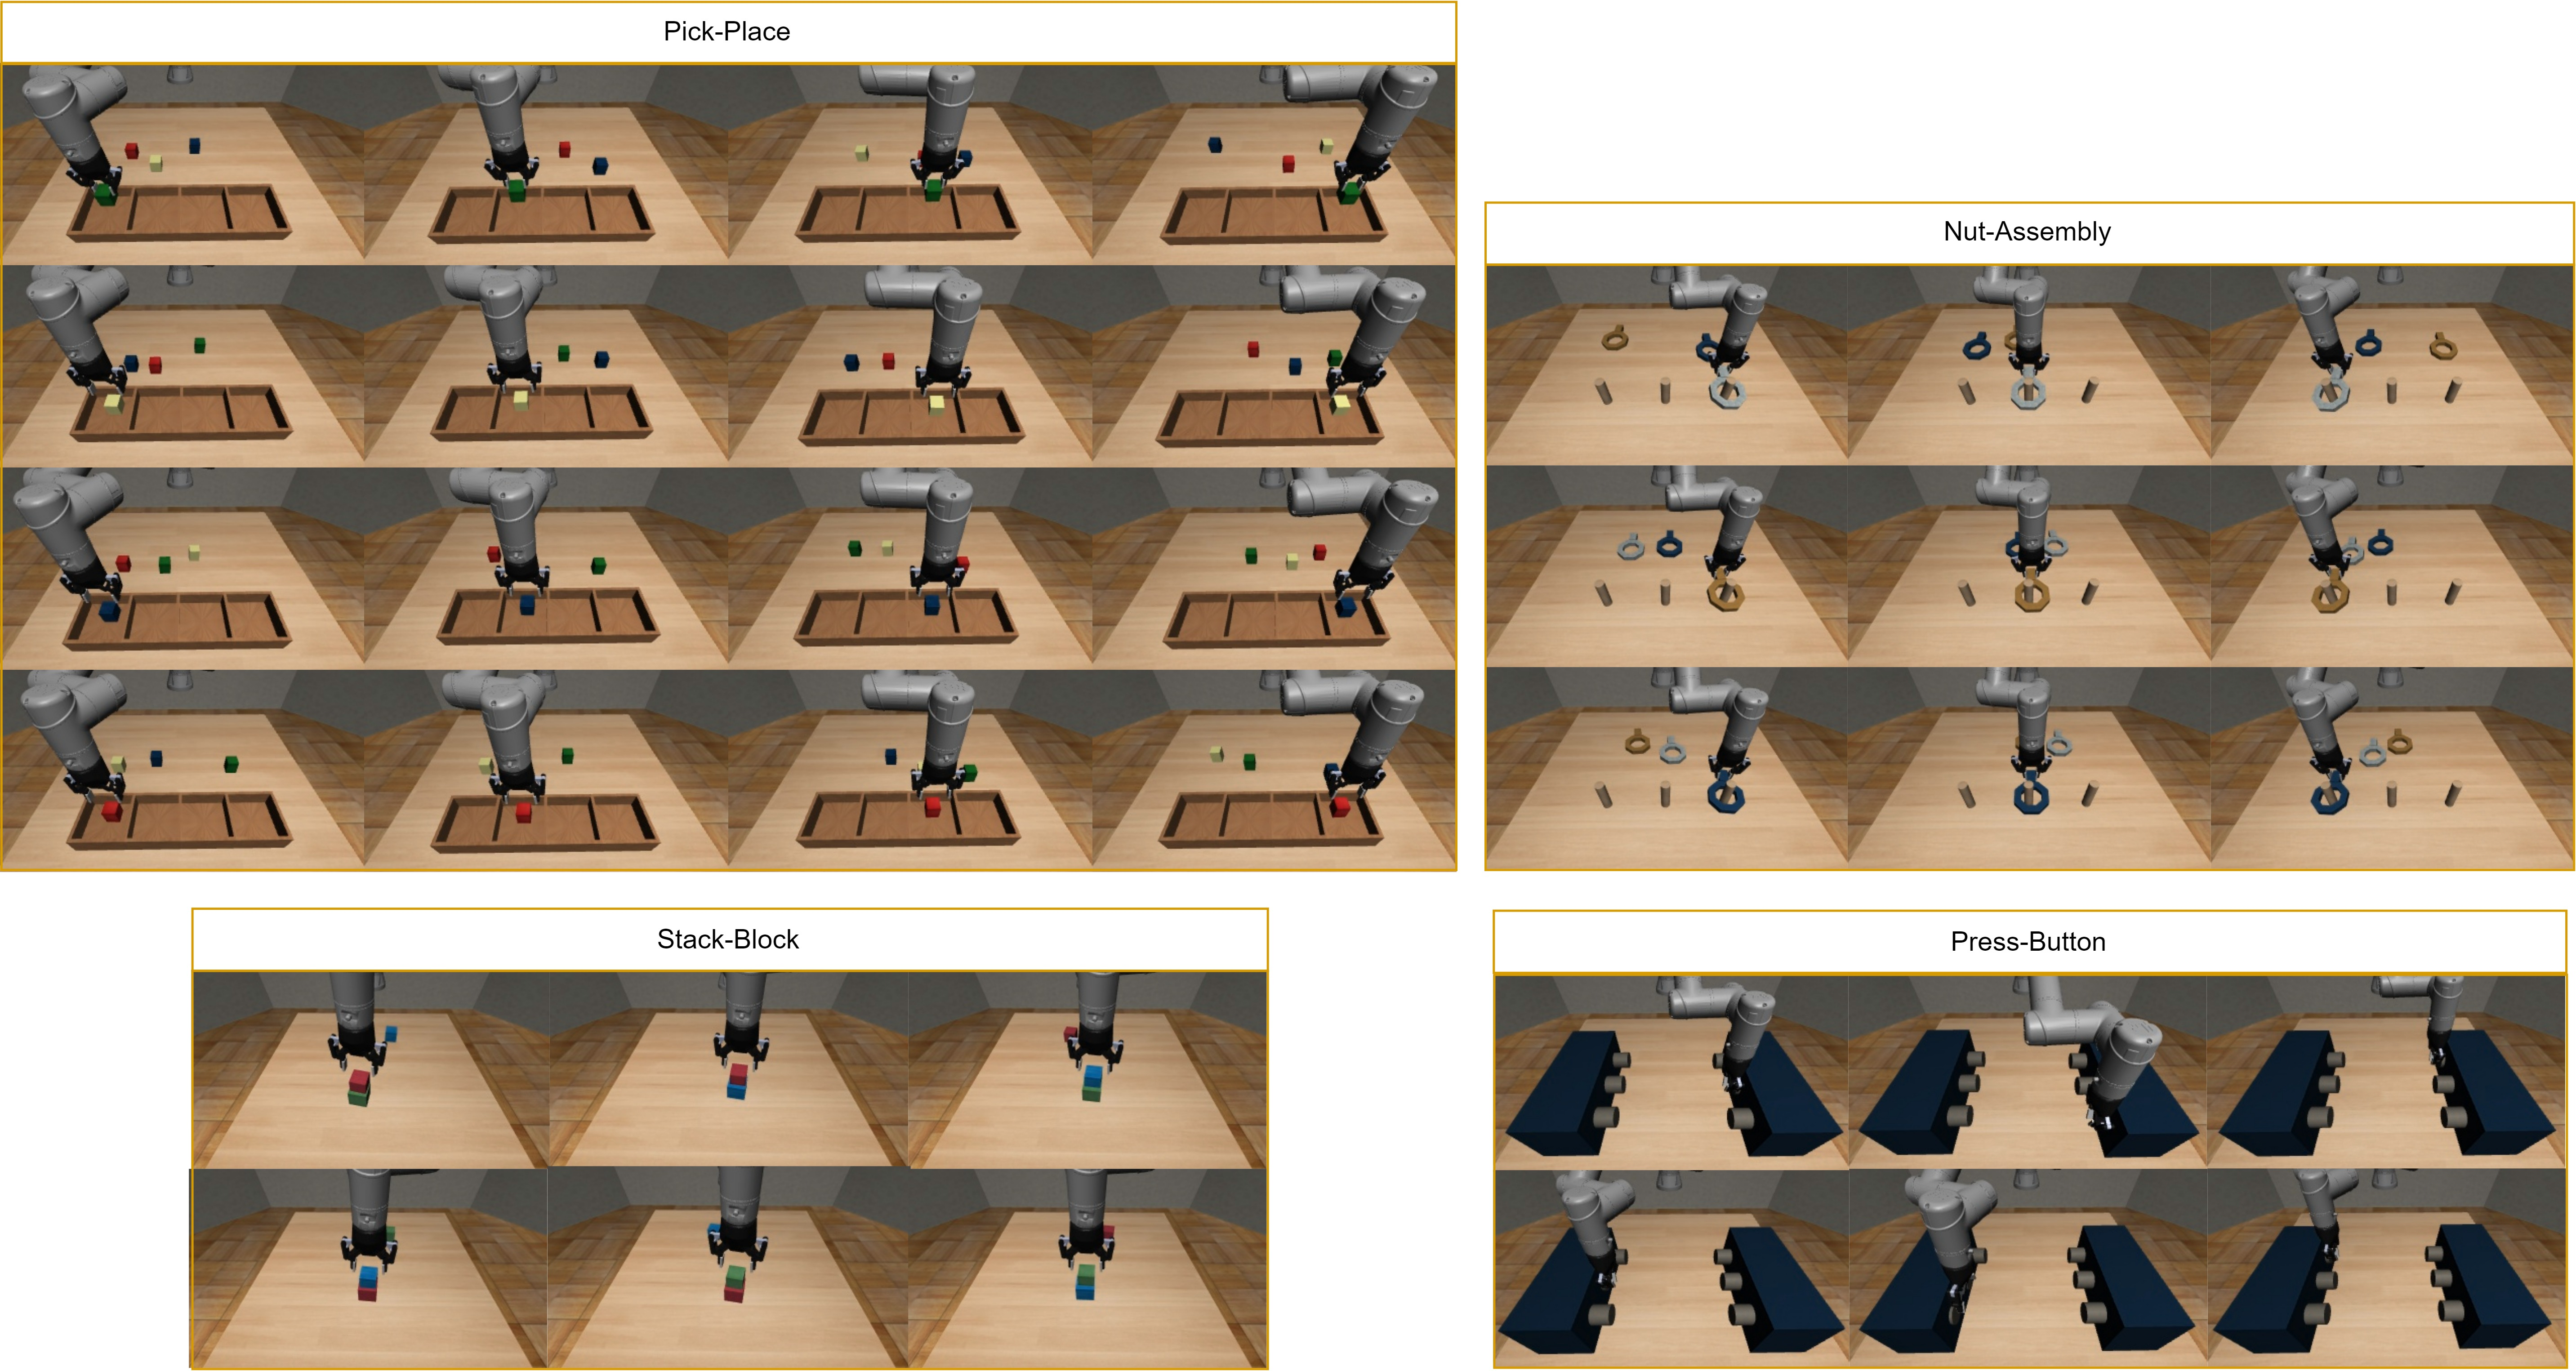
\includegraphics[width=1.0\textwidth]{figures/images/ch2/dataset.jpg}
    \caption{Examples of tasks and variations taken in consideration for the methods validation. The images report the final system state. For the pick-place, nut-assembly and stack-block tasks the variation is defined with respect to the target object and the placing location, while for the press-button the variation is defined according to the button to press.}
    \label{fig:dataset_cod}
\end{figure}


For each task, 100 trajectories were collected for both the agent (UR5e robot) and the demonstrator (Franka-Emika Panda robot) using hand-written policies that take as input ground-truth information about the object position. Across these trajectories, the position of the objects of interest varies. The workspace for each task is divided as follows:
\begin{itemize}
    \item \textbf{Pick-Place}: The bins are fixed in position, while the boxes can change according to the following rule. The workspace is divided into 4 slots, parrallel to the bins, each with a width of $6 \ \text{cm}$ and a height of $15 \ \text{cm}$. A slot is randomly selected, and the box is randomly spawned within the chosen slot, ensuring that each slot is filled with only one object.
    \item \textbf{Nut-Assembly}: The pegs are fixed in position, while the nuts vary in placement. A spawn region of $75 \times 10 \ \text{cm}$ is defined, and the nuts are randomly spawned in this region, ensuring they do not collide with one another.
    \item \textbf{Stack-Block}: The placing box is spawned in a region of $16 \times 5 \ \text{cm}$, while the target box is spawned in a region of $24 \times 5 \ \text{cm}$, ensuring no collisions between the boxes.
    \item \textbf{Press-Button}: The two sets of buttons are placed within a region of $4 \times 4 \ \text{cm}$.
\end{itemize}

The bounding-boxes are automatically generated. The procedure followed to generate the bounding boxes assume the knowledge of the pose and dimention of the object, as well as the knowledge of the pose of the camera and its intrinsic parameters. Giving all these information, it is possible to build a 3D bounding-box around the object in the continous world space, then project the corners in the 2D discrete camera space through a sequence of transformations described in Formula \ref{}.
\begin{equation}
\end{equation}
\smalltodo{add equation}
\subsection{Results}
\label{sec:cod_results}
This section presents the obtained results, divided into two main blocks. The first block (Section~\ref{sec:cod_tod}) discusses the results of the method trained to detect only the target object. The second block (Section~\ref{sec:cod_tod}) covers the results of the method trained to detect both the target object and the final (placing) location. For each method, results are reported for two different scenarios: first, where the method is trained in a single-task multi-variation scenario; and second, where the method is trained in a multi-task multi-variation scenario.

For all the test configurations described below, the testing procedure was consistent. Specifically, for each task and its variations, 10 rollouts were performed. During each rollout, the robot was controlled by a hand-written policy, and the predicted bounding box was compared with the ground truth, obtained using the same procedure as described earlier.

The metrics used to evaluate the methods were \textit{Precision@0.5} (Equation \ref{eq:prec}) and \textit{Recall@0.5} (Equation \ref{eq:rec}).
\begin{equation}
    \label{eq:prec}
    Pre = \frac{TP}{TP+FP}
\end{equation} 
\begin{equation}
    \label{eq:rec}
    Rec = \frac{TP}{TP+FN}
\end{equation}

A \textit{True Positive} (TP) sample is defined as a predicted bounding box for the target class with an Intersection over Union (IoU) greater than or equal to 0.5 when compared with the ground-truth bounding box. A \textit{False Positive} (FP) sample is defined as a predicted bounding box for the target class with an IoU less than 0.5. A \textit{False Negative} (FN) sample is defined as a target object for which no bounding box was predicted.

The metrics were computed considering only the target bounding boxes, i.e., the bounding boxes predicted for the target object or the target location. Among all the candidates generated by the network, only the one with the highest predicted class score was considered.


\subsubsection{Target object detector}
This first set of validation tests is related to the training of the COD module in a setting where it must predict the location of the target-object. This means that, with respect to the semantic attributes defined in Section \ref{sec:cod_problem}, the set is restricted to just two classes ``target'' and ``no-target''. In this case, the method will be named \textit{Conditioned Target Object Detector} (CTOD).
\label{sec:cod_tod}
\paragraph*{Single-task multi-variation scenario}\mbox{}\\
In the single-task multi-variation scenario, a specific model was trained for each task described in Figure \ref{fig:dataset_cod}. This approach allows for evaluating the model ability to handle tasks of increasing complexity. Initially, the model is evaluated in a simpler scenario, where it predicts the target position of a specific category of objects (e.g., only boxes in pick-and-place, or only nuts in nut-assembly), thereby limiting variability in object categories.
% \usepackage{graphicx}
% \usepackage{hhline}

% \usepackage{hhline}


% \usepackage{graphicx}
% \usepackage{hhline}


\begin{table}[t]
    \centering
    \caption{Results of the CTOD module obtained in the single-task multi-variation scenario. Performances are reported in terms of \textit{Precision} (Prec), \textit{Recall} (Rec) with an IoU threshold of 0.5 and the Average IoU $(IoU_{avg})$ }
    \label{table:ctod_single_task_performance}
    \begin{tabular}{|c|c|c|c|} 
    \hline
    \textbf{Task} & \textbf{Precision@0.5} & \textbf{Recall@0.5} & $\mathbf{IoU_{avg}}$ \\ 
    \hhline{|====|}
    Pick-Place & 0.770 & 1.00 & 0.628 \\ 
    \hline
    Nut-Assembly & 0.985 & 1.00 & 0.789 \\ 
    \hline
    Stack-Block & 0.995 & 1.00 & 0.848 \\ 
    \hline
    Press-Button & 0.997 & 1.00 & 0.899 \\
    \hline
    \end{tabular}
    \end{table}

% \begin{table}[t]
%     \centering
%     \refstepcounter{table}
%     \caption{Distribution of the predicted bounding boxes generated by the CTOD module in the single-task, multi-variation scenario.}
%     \label{table:ctdo_single_task_prediction_distribution}
%     \resizebox{\linewidth}{!}{%
%     \begin{tabular}{|c|c|c|c|c|c|} 
%     \hline
%     \textbf{Task} & \textbf{TP} & \begin{tabular}[c]{@{}c@{}}\textbf{FP }\\\textbf{pre-picking}\end{tabular} & \begin{tabular}[c]{@{}c@{}}\textbf{FP }\\\textbf{post-picking}\end{tabular} & \begin{tabular}[c]{@{}c@{}}\textbf{FN }\\\textbf{pre-picking}\end{tabular} & \begin{tabular}[c]{@{}c@{}}\textbf{FN }\\\textbf{post-picking}\end{tabular} \\ 
%     \hhline{|======|}
%     \begin{tabular}[c]{@{}c@{}}Pick-Place \\(XXXX)\end{tabular} & XXXX & XXXX & XXXX & XXXX & XXXX \\ 
%     \hline
%     \begin{tabular}[c]{@{}c@{}}Nut-Assembly \\(XXXX)\end{tabular} & XXXX & XXXX & XXXX & XXXX & XXXX \\ 
%     \hline
%     \begin{tabular}[c]{@{}c@{}}Stack-Block\\(XXXX)\end{tabular} & XXXX & XXXX & XXXX & XXXX & XXXX \\ 
%     \hline
%     \begin{tabular}[c]{@{}c@{}}Press-Button\\(XXXX)\end{tabular} & XXXX & XXXX & XXXX & XXXX & XXXX \\
%     \hline
%     \end{tabular}
%     }
%     \end{table}

\begin{table}[t]
\centering
\caption{Results of the CTOD module obtained in the multi-task multi-variation scenario. Performances are reported in terms of \textit{Precision} (Prec), \textit{Recall} (Rec) with an IoU threshold of 0.5 and the Average IoU $(IoU_{avg})$}
\label{table:ctod_multi_task_performance}
\begin{tabular}{|c|c|c|c|} 
\hline
\textbf{Task} & \textbf{Precision@0.5} & \textbf{Recall@0.5} & $\mathbf{IoU_{avg}}$ \\ 
\hhline{|====|}
Pick-Place & 0.652 & 1.00 & 0.563 \\ 
\hline
Nut-Assembly & 0.948 & 1.00 & 0.726 \\ 
\hline
Stack-Block & 0.894 & 1.00 & 0.708 \\ 
\hline
Press-Button & 0.977 & 1.00 & 0.825 \\
\hline
\end{tabular}
\end{table}

% \begin{table}[t]
%     \centering
%     \refstepcounter{table}
%     \caption{Distribution of the predicted bounding boxes generated by the CTOD module in the multi-task, multi-variation scenario.}
%     \label{table:ctdo_multi_task_prediction_distribution}
%     \resizebox{\linewidth}{!}{%
%     \begin{tabular}{|c|c|c|c|c|c|} 
%     \hline
%     \textbf{Task} & \textbf{TP} & \begin{tabular}[c]{@{}c@{}}\textbf{FP }\\\textbf{pre-picking}\end{tabular} & \begin{tabular}[c]{@{}c@{}}\textbf{FP }\\\textbf{post-picking}\end{tabular} & \begin{tabular}[c]{@{}c@{}}\textbf{FN }\\\textbf{pre-picking}\end{tabular} & \begin{tabular}[c]{@{}c@{}}\textbf{FN }\\\textbf{post-picking}\end{tabular} \\ 
%     \hhline{|======|}
%     \begin{tabular}[c]{@{}c@{}}Pick-Place \\(XXXX)\end{tabular} & XXXX & XXXX & XXXX & XXXX & XXXX \\ 
%     \hline
%     \begin{tabular}[c]{@{}c@{}}Nut-Assembly \\(XXXX)\end{tabular} & XXXX & XXXX & XXXX & XXXX & XXXX \\ 
%     \hline
%     \begin{tabular}[c]{@{}c@{}}Stack-Block\\(XXXX)\end{tabular} & XXXX & XXXX & XXXX & XXXX & XXXX \\ 
%     \hline
%     \begin{tabular}[c]{@{}c@{}}Press-Button\\(XXXX)\end{tabular} & XXXX & XXXX & XXXX & XXXX & XXXX \\
%     \hline
%     \end{tabular}
%     }
%     \end{table}
Table \ref{table:ctod_single_task_performance} presents the overall performance of the CTOD module in terms of Precision and Recall, providing a comprehensive evaluation of the system ability to accurately identify target objects (Precision) and consistently detect them across multiple rollouts (Recall). The results demonstrate that the module successfully identifies target objects with precise bounding boxes and maintains a high level of consistency across rollouts, achieving excellent precision and recall metrics. 

In particular, the Recall remains consistently at \textbf{1.00}, indicating the absence of false negatives, meaning the system always generates a bounding box classified as the ``target" object. Precision values are also high, exceeding \textbf{0.90} for three tasks: Nut-Assembly, Stack-Block, and Press-Button. However, a lower Precision is observed for the Pick-Place task. This is due to the task longer motion duration, both in terms of time and space, which introduces varying scales of the target object throughout the motion, increasing the complexity of predicting accurate bounding boxes. Specifically, out of the 2612 false positives generated for the Pick-Place task, \textbf{2125} were produced after the picking phase, while only \textbf{487} occurred during the reaching phase.

Generally, the obtained performance demonstrate that the module not only generates bounding boxes with the correct ``target" classification but also produces highly accurate bounding boxes that closely match the ground truth. Figure \ref{fig:ctod_example_of_prediction} shows examples of predictions for all tasks during the execution of a rollout. As observed, during the approaching phase, crucial for avoiding target misidentification, the bounding box remains accurately positioned around the target object. However, during the robot motion, the bounding box slightly shifts, occasionally resulting in false positives.

\begin{figure}[t]
    \centering
    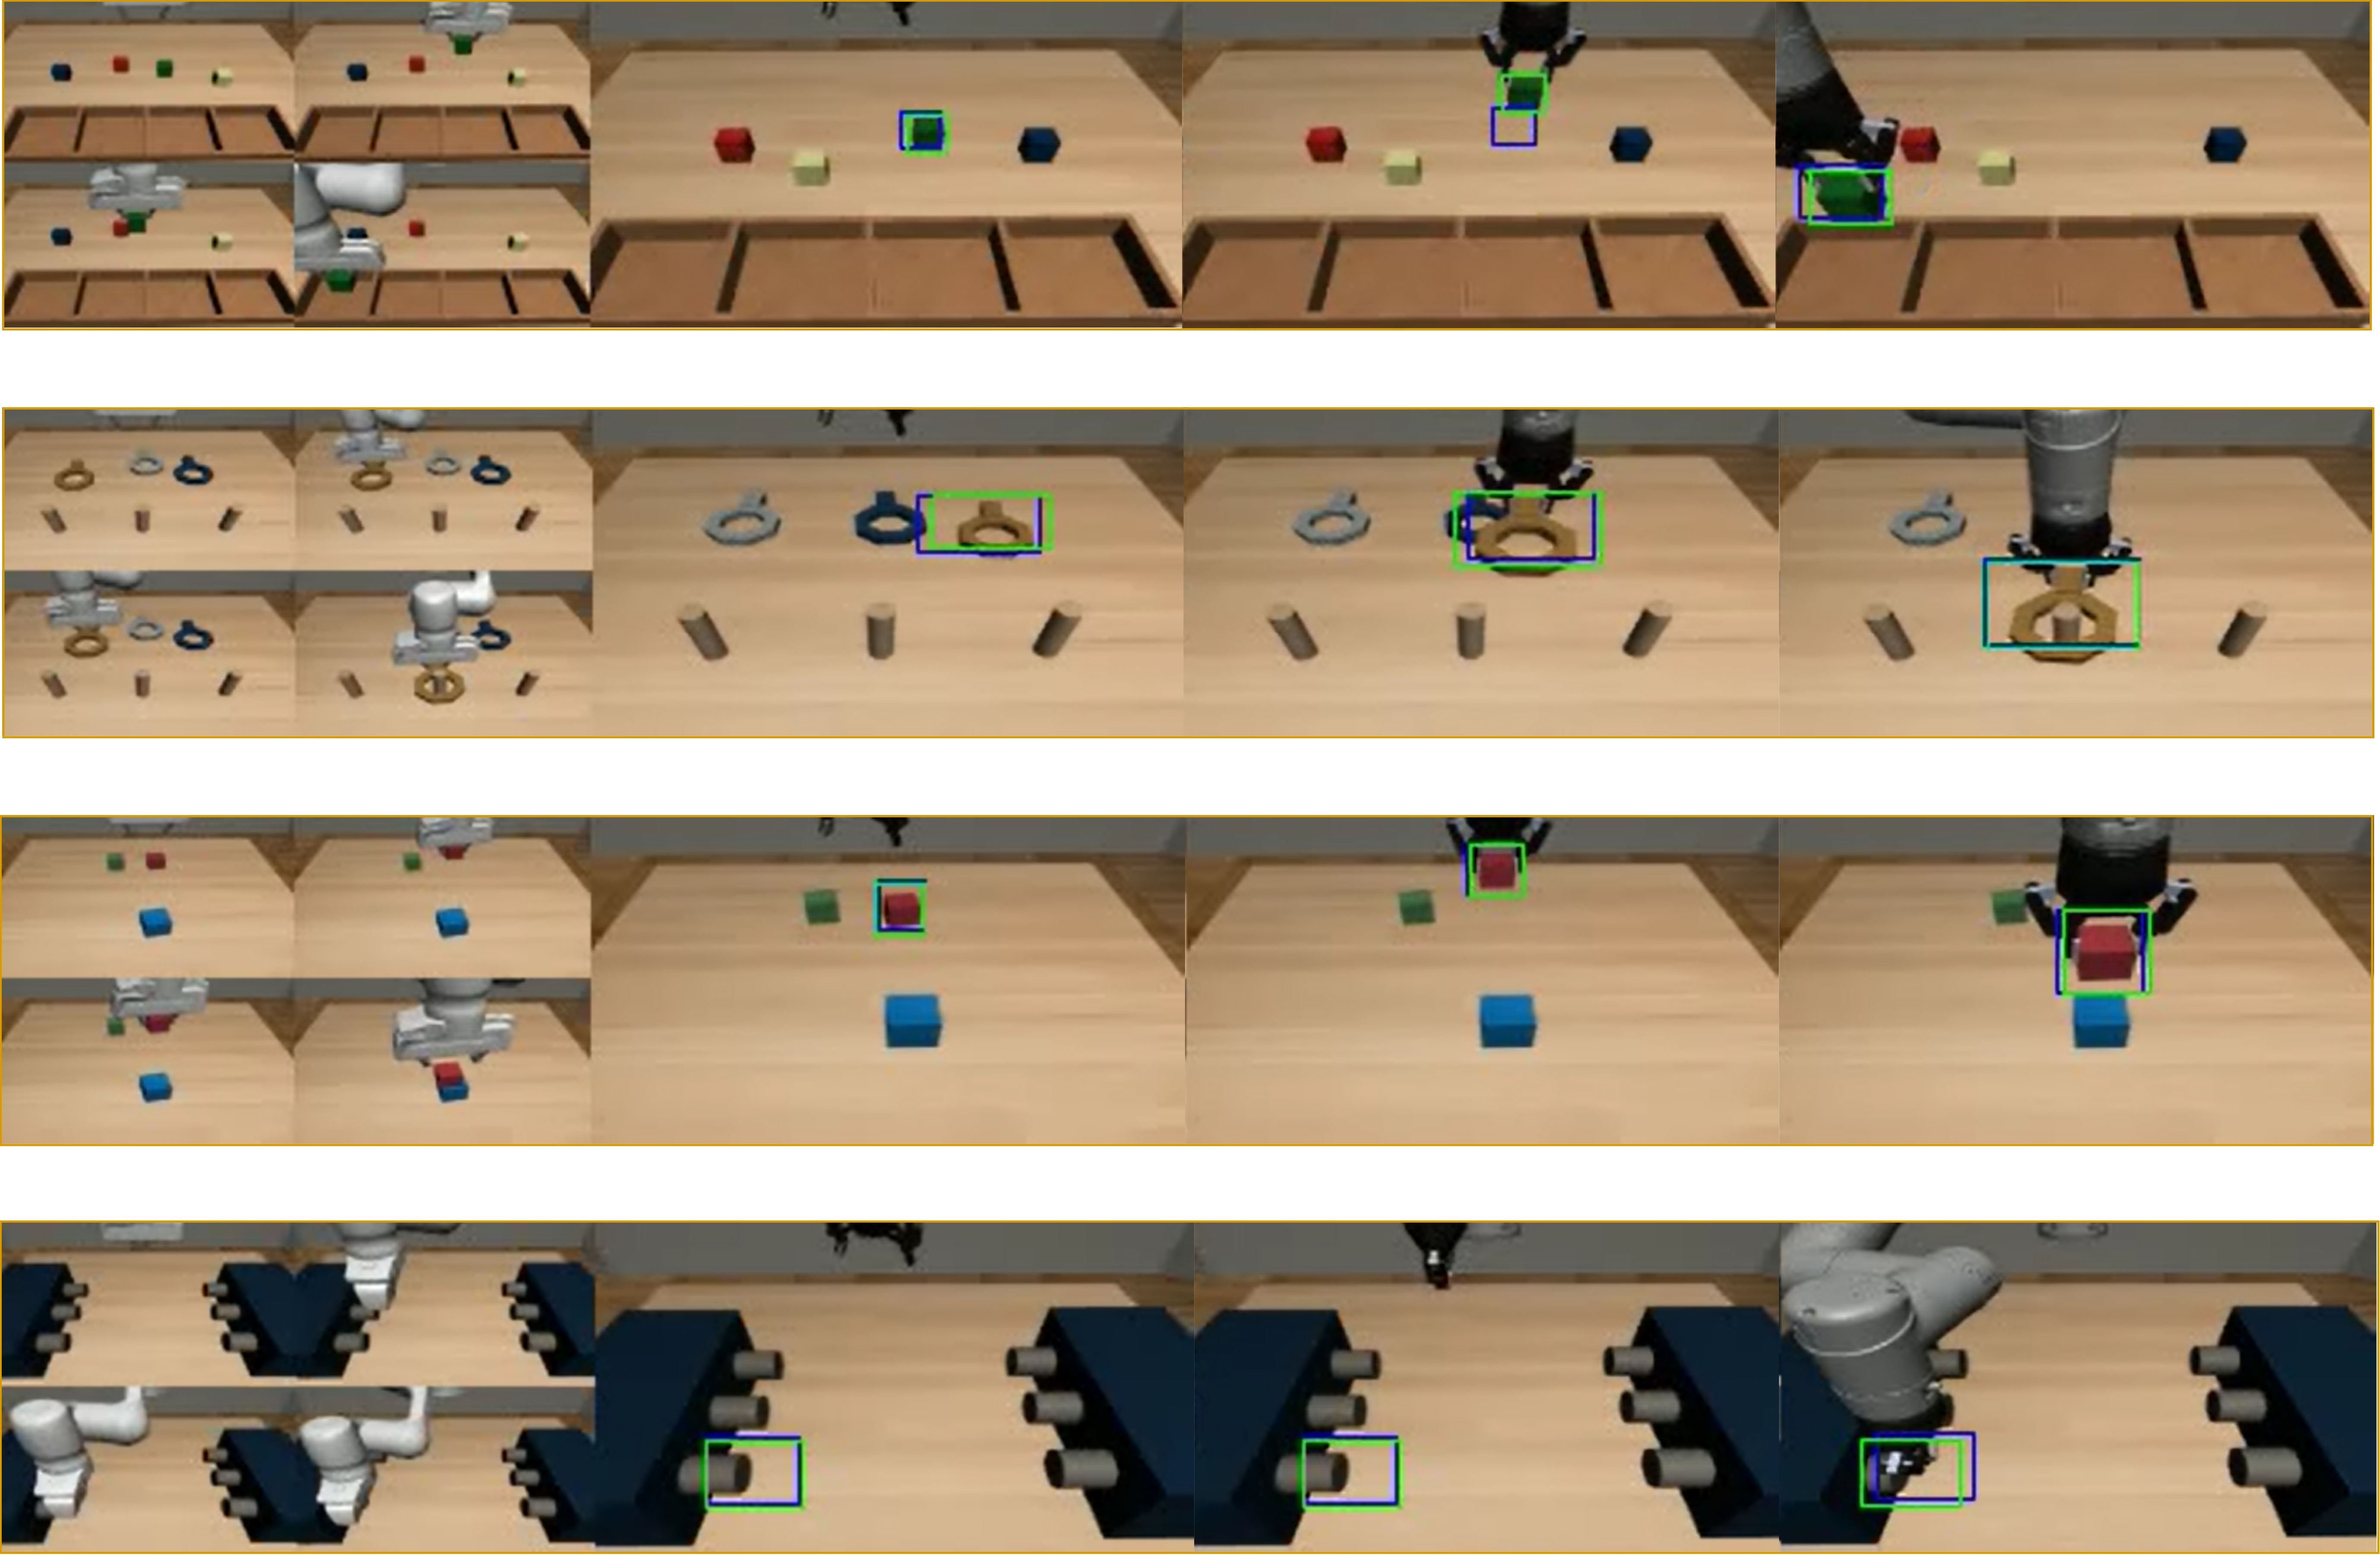
\includegraphics[width=1.0\textwidth]{figures/images/ch2/example_of_prediction_ctod_single.jpg}
    \caption{Example of predictions generated by the CTOD module in the single-task scenario. The blue-box is the predicted one, while the green is the ground truth.}
    \label{fig:ctod_example_of_prediction}
\end{figure}


\paragraph*{Multi-task multi-variation scenario}\mbox{}\\
In the multi-task multi-variation scenario, a single model was trained to perform all four tasks. This setup enables a more rigorous validation of the COD module in a complex environment, where objects of different shapes and sizes are involved across various tasks. Table \ref{table:ctod_multi_task_performance} presents the overall performance of the COD module in terms of Precision and Recall. In this scenario, the system consistently generates bounding boxes for the "target" class (achieving a Recall of 1.00 for all tasks) with an average overlap greater than 0.5. A similar trend as in the single-task scenario is observed, with a lower Precision for the Pick-Place task due to the same reasons previously explained.

Furthermore, compared to the single-task setting, a slight reduction in Average IoU is observed, which can be attributed to the increased complexity of the task. In this multi-task scenario, a single Fast R-CNN must predict bounding boxes across a diverse set of manipulation tasks, where objects may be similar but appear at different scales in the input images. This variation adds further complexity to the prediction process.


\subsubsection{Target object and final position detector}
\label{sec:cod_tofpd}
This set of validation tests focuses on training the COD module in the complete scenario described in Section \ref{sec:cod_problem}. In this setting, the COD module is trained to predict bounding boxes for both the target object and the final location of interest. Specifically, for the three tasks involving the ``pick-and-place" primitive (i.e., Pick-Place, Nut-Assembly, and Stack-Block), the final location corresponds to the target bin, peg, and block to be stacked, respectively. In contrast, for the Press-Button task, the target location is defined as the bounding box of the initial button, translated to the final position of the pressed button (Figure \ref{fig:press_button_target_placing}).
\begin{figure}[t]
    \centering
    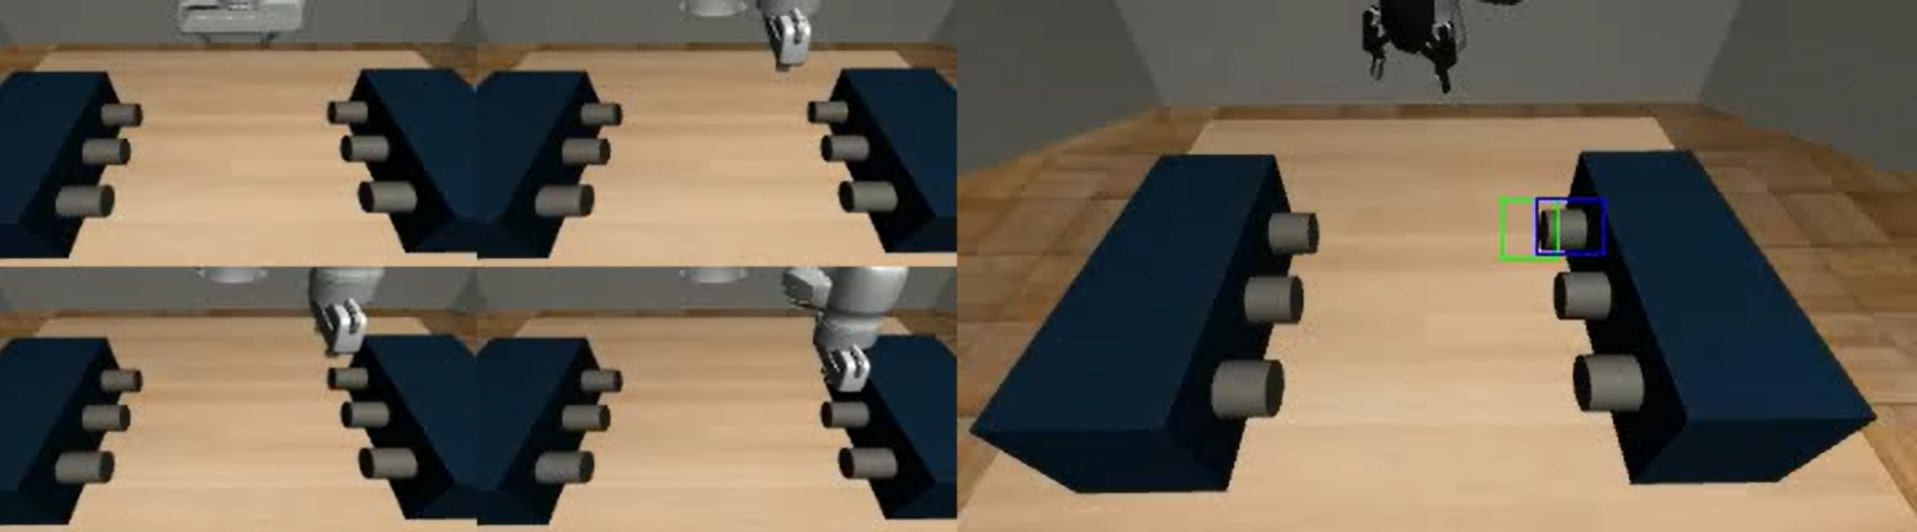
\includegraphics[width=0.9\textwidth]{figures/images/ch2/press_button_target_placing.jpg}
    \caption{Example of Target Bounding Box and Final Placing Position Definition for the Press-Button Task. In this task, the target bounding box is represented by the green bounding box, which encloses the button that needs to be pressed. The blue bounding box represents the final placing position, indicating the location where the robot's end-effector should be positioned to successfully press the button.}
    \label{fig:press_button_target_placing}
\end{figure}


\begin{table}[t]
    \centering
    \caption{Results of the COD module obtained in the single-task multi-variation scenario. Performances are reported in terms of \textit{Precision} (Prec), \textit{Recall} (Rec) with an IoU threshold of 0.5 and the Average IoU $(IoU_{avg})$ for both the bounding-box of the ``target" and the ``target-place" classes.}
    \label{table:cod_single_task_performance}
    \resizebox{\linewidth}{!}{%
    \begin{tabular}{|c|c|c|c|c|} 
    \hline
    \textbf{Task} & \textbf{Precision@0.5} & \textbf{Recall@0.5} & \begin{tabular}[c]{@{}c@{}}$\mathbf{IoU_{avg}}$~\\(target)\end{tabular} & \begin{tabular}[c]{@{}c@{}}$\mathbf{IoU_{avg}}$~\\(target-place)\end{tabular} \\ 
    \hhline{|=====|}
    Pick-Place & 0.667 & 1.00 & 0.374 & 0.826 \\ 
    \hline
    Nut-Assembly & 0.958 & 1.00 & 0.705 & 0.909 \\ 
    \hline
    Stack-Block & 0.979 & 1.00 & 0.787 & 0.827 \\ 
    \hline
    Press-Button & 0.967 & 1.00 & 0.799 & 0.683 \\
    \hline
    \end{tabular}
    }
    \end{table}
% \begin{table}[t]
%     \centering
%     \refstepcounter{table}
%     \caption{Distribution of the predicted bounding boxes generated by the CTOD module in the single-task, multi-variation scenario.}
%     \label{table:ctdo_single_task_prediction_distribution}
%     \resizebox{\linewidth}{!}{%
%     \begin{tabular}{|c|c|c|c|c|c|} 
%     \hline
%     \textbf{Task} & \textbf{TP} & \begin{tabular}[c]{@{}c@{}}\textbf{FP }\\\textbf{pre-picking}\end{tabular} & \begin{tabular}[c]{@{}c@{}}\textbf{FP }\\\textbf{post-picking}\end{tabular} & \begin{tabular}[c]{@{}c@{}}\textbf{FN }\\\textbf{pre-picking}\end{tabular} & \begin{tabular}[c]{@{}c@{}}\textbf{FN }\\\textbf{post-picking}\end{tabular} \\ 
%     \hhline{|======|}
%     \begin{tabular}[c]{@{}c@{}}Pick-Place \\(XXXX)\end{tabular} & XXXX & XXXX & XXXX & XXXX & XXXX \\ 
%     \hline
%     \begin{tabular}[c]{@{}c@{}}Nut-Assembly \\(XXXX)\end{tabular} & XXXX & XXXX & XXXX & XXXX & XXXX \\ 
%     \hline
%     \begin{tabular}[c]{@{}c@{}}Stack-Block\\(XXXX)\end{tabular} & XXXX & XXXX & XXXX & XXXX & XXXX \\ 
%     \hline
%     \begin{tabular}[c]{@{}c@{}}Press-Button\\(XXXX)\end{tabular} & XXXX & XXXX & XXXX & XXXX & XXXX \\
%     \hline
%     \end{tabular}
%     }
%     \end{table}

\begin{table}[t]
    \centering
    \caption{Results of the COD module obtained in the multi-task multi-variation scenario. Performances are reported in terms of \textit{Precision} (Prec), \textit{Recall} (Rec) with an IoU threshold of 0.5 and the Average IoU $(IoU_{avg})$ for both the bounding-box of the ``target'' and the ``target-place'' classes.}
    \label{table:cod_multi_task_performance}
    \resizebox{\linewidth}{!}{%
    \begin{tabular}{|c|c|c|c|c|} 
    \hline
    \textbf{Task} & \textbf{Precision@0.5} & \textbf{Recall@0.5} & \begin{tabular}[c]{@{}c@{}}$\mathbf{IoU_{avg}}$ \\~(target)\end{tabular} & \begin{tabular}[c]{@{}c@{}}$\mathbf{IoU_{avg}}$~\\(target-place)\end{tabular} \\ 
    \hhline{|=====|}
    Pick-Place & 0.735 & 1.00 & 0.457 & 0.825 \\ 
    \hline
    Nut-Assembly & 0.951 & 1.00 & 0.685 & 0.898 \\ 
    \hline
    Stack-Block & 0.867 & 1.00 & 0.628 & 0.799 \\ 
    \hline
    Press-Button & 0.925 & 1.00 & 0.734 & 0.687 \\
    \hline
    \end{tabular}
    }
    \end{table}
% \begin{table}[t]
%     \centering
%     \refstepcounter{table}
%     \caption{Distribution of the predicted bounding boxes generated by the CTOD module in the multi-task, multi-variation scenario.}
%     \label{table:ctdo_multi_task_prediction_distribution}
%     \resizebox{\linewidth}{!}{%
%     \begin{tabular}{|c|c|c|c|c|c|} 
%     \hline
%     \textbf{Task} & \textbf{TP} & \begin{tabular}[c]{@{}c@{}}\textbf{FP }\\\textbf{pre-picking}\end{tabular} & \begin{tabular}[c]{@{}c@{}}\textbf{FP }\\\textbf{post-picking}\end{tabular} & \begin{tabular}[c]{@{}c@{}}\textbf{FN }\\\textbf{pre-picking}\end{tabular} & \begin{tabular}[c]{@{}c@{}}\textbf{FN }\\\textbf{post-picking}\end{tabular} \\ 
%     \hhline{|======|}
%     \begin{tabular}[c]{@{}c@{}}Pick-Place \\(XXXX)\end{tabular} & XXXX & XXXX & XXXX & XXXX & XXXX \\ 
%     \hline
%     \begin{tabular}[c]{@{}c@{}}Nut-Assembly \\(XXXX)\end{tabular} & XXXX & XXXX & XXXX & XXXX & XXXX \\ 
%     \hline
%     \begin{tabular}[c]{@{}c@{}}Stack-Block\\(XXXX)\end{tabular} & XXXX & XXXX & XXXX & XXXX & XXXX \\ 
%     \hline
%     \begin{tabular}[c]{@{}c@{}}Press-Button\\(XXXX)\end{tabular} & XXXX & XXXX & XXXX & XXXX & XXXX \\
%     \hline
%     \end{tabular}
%     }
%     \end{table}
\paragraph*{Single-task multi-variation scenario}\mbox{}\\
Table \ref{table:cod_single_task_performance} summarizes the performance of the COD module in the single-task, multi-variation evaluation setting. It can be observed that, even in this scenario, the COD module consistently identifies both the target object and the target placement location. Specifically, the average Intersection over Union ($IoU_{avg}$) is generally higher for the target-placement class. This is because, for the Pick-Place, Nut-Assembly, and Stack-Block tasks, the placement location is fixed, making the detection problem easier for the conditioning module to address. 

Regarding the ``target" class, the $IoU_{avg}$ is lower compared to Table \ref{table:ctod_single_task_performance}, with a significant drop observed in the Pick-Place task. However, by examining the distribution of false positives, it can be noted that, out of \textbf{7565} false-positive cases, \textbf{2001} occurred during the reaching phase, while the remaining \textbf{5564} occurred during the placing phase. 

It is worth noting that the module can still identify the region of the target object. In fact, by lowering the IoU threshold to 0.1, the number of false positives during the reaching phase drops to 155, indicating that the system is able to detect the region of interest, albeit with lower precision. Nevertheless, for the task at hand, having consistently precise bounding boxes is not critical, as the control module is designed to be robust against minor errors or imprecisions in bounding box predictions.


\paragraph*{Multi-task multi-variation scenario}\mbox{}\\
The final evaluation setting essentially confirms the trends observed in the previous one. Table \ref{table:cod_multi_task_performance} summarizes the results obtained from the COD module trained in the multi-task scenario. In this case, a slight drop in Precision is again observed, which corresponds to a decrease in the average Intersection over Union ($IoU_{avg}$). This decline can be attributed to the same reasons discussed in the previous multi-task setting, with the added complexity that the module must also predict the bounding box for the target placement location.


In conclusion, this paragraph has introduced the COD module, a Conditioned-Convolutional Neural Network designed to address a novel object-detection problem. The module predicts category-agnostic bounding boxes for the two key regions in a manipulation task: the region where the object to be manipulated is located and the final region where the task is completed (e.g., placing the box, assembling the nut, stacking the block, or pressing the button). In a highly generalized multi-variation scenario, where the object position is not predefined and the semantic attribute assigned to the object is dynamically specified by a command, which is given through a video demonstration of another agent performing the desired task.


The results demonstrate that the proposed module effectively handles both single-task and multi-task scenarios, generating bounding boxes that are correctly classified and accurately identify the regions of interest.

In Chapter \ref{ch:occp}, it will be shown how the positional information from this command can be effectively utilized to inform the control module about the regions of interest, addressing the problem of target misidentification.


\section{Conclusion}
In conclusion, this chapter introduced and discussed the Conditioned Object Detector (COD), representing a foundational step toward a modular architecture for Visual-Conditioned \\ Multi-Task Imitation Learning. This module tackles a critical aspect of cognitive task design: dynamically identifying the region of interest within an agent scene based on a demonstrated task. Its primary objective is to identify the relevant target object and its final placement location in scenarios involving multiple potential objects and placement options. The specific semantic roles of these objects (i.e., target or distractor) are determined at runtime through the provided task demonstration.

To tackle this challenge, a conditioned convolutional architecture was introduced and tested in both single-task multi-variation and multi-task multi-variation scenarios.

The results demonstrated that the proposed COD architecture effectively identified objects of interest, consistently achieving a Recall@0.5 score of \textbf{1.00} across all tasks and testing scenarios. This means that for every frame, a bounding box corresponding to the target class was always present.

Regarding Precision@0.5, there was variability across different tasks and scenarios, ranging from a minimum of \textbf{0.652} for the Pick-Place task in the multi-task multi-variation scenario to a maximum of \textbf{0.997} for the Press-Button task in the single-task multi-variation scenario. Despite this variation, the system was able to consistently identify the target object, with an average IoU always greater than 0.3. While this might appear low, further analysis of the generated bounding boxes revealed that the system successfully identified the target object during the initial stages of the rollout, particularly in the reaching phase, when conditioning on the target object is critical. However, a notable number of false positives occurred during the manipulation and placing phases, where the conditioning on the target object weakens, suggesting that the trained policy must be robust to errors in bounding box generation during these phases.